
\subsection{Comparación entre secuencial, vectorial y multicore}
Ya analizado el tipo de mejoras que son implementadas por G++ al utilizar -O1, -O2 y -O3, se presentan en esta sección los resultados de los experimentos realizados. Se comparan mediciones de tiempo de los distintos flags presentes en el compilador, con otras técnicas. 
~\\
~\\
En particular se estudian los flags -O0, -O1, -O2, -O3 y -Ofast del compilador GCC (GNU Compiler Colection), -O0, -O1, -O2, -O3 y -Ofast para ICC (Intel C++ Compiler), -O0, -O1, -O2, -O3 y -Ofast para GCC, peor utilizando OpenMP, y por último -O0, -O3 y -Ofast para la versión vectorizada desarrollada en este trabajo, la cual consta de una parte en C++ en comun con la versión no vectorial, que fue compilada con GCC, y una función implementada en Assembler y compilada mediante NASM (Netwide Assembler x86), especificamente desarrollada para aprovechar la tecnología SIMD, y seleccionada por ser la sección mas critica en terminos de rendimiento, del programa original.
~\\
~\\
Para cada técnica se experimentó con distintos tamaños del sistema simulado, comenzando desde simulaciónes de sistemas pequeños de 1x1$m^2$ y aumentando de a un metro el lado del sistema, hasta llegar a 20x20$m^2$, el tamaño de lado es además la medida correspondiente al eje horizontal, mientras que el tiempo medido en segundos, es el correspondiente al eje vertical. Además, para cada punto, se realizaron 100 repticiónes, y se tomo la media y desvio estándar de las mismas, con el objetivo de eliminar el error de medición introducido por la falta de control del tiempo otorgado a las distintas tareas del sistema operativo por parte del scheduler. 
~\\
~\\
Los tiempos fueron medidos mediante la utilización de la herramienta time de Linux, bajo la distribución Ubuntu 16.04 LTS, en una maquina i7-920 2.67GHz, 18GB ram, 1TB HDD 7200rpm. Además no se utilizó la maquina durante la experimentación, para no introducir ruido en las mediciónes. En total se realizaron cerca de 40.000 simulaciónes. A continuación se muestran los resultados de las mismas.
~\\
~\\
Se mostrarán primero los datos obtenidos para GCC, en particular su compilador C++, para distintos niveles de optimización.
~\\
~\\
\begin{figure}[H]
\caption{Tiempo(s) vs Tamaño(m) para GCC}
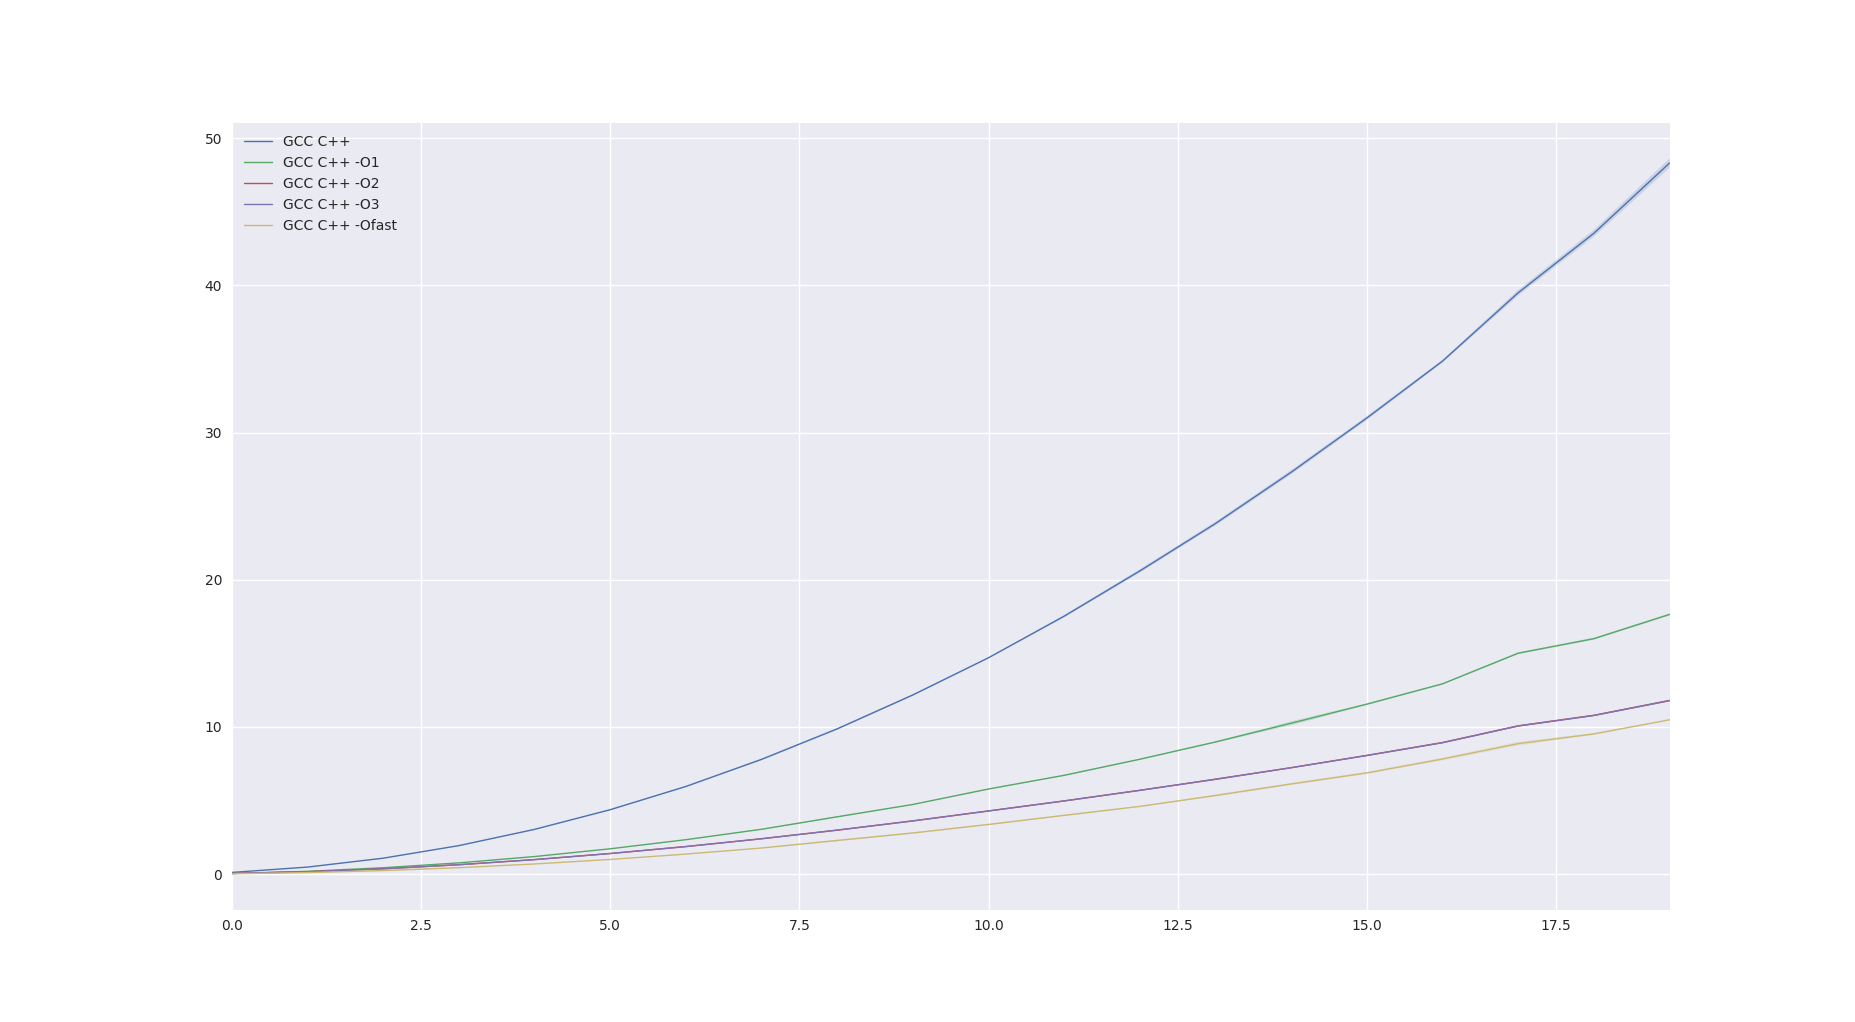
\includegraphics[width=\textwidth]{imagenes/plot_cpp.png}
\end{figure}
~\\
~\\
Como es de esperar, el programa responde bien a las mejoras, con la mayor diferencia dandose entre -O0 y -O1, y la menor entre -O3 y -Ofast. Para el caso de mayor tamaño, el programa, distando de tardar casi 50s como en -O0, da un resultado menor a 20s, un tiempo menor a la mitad.
~\\
~\\
\begin{figure}[H]
\caption{Tiempo(s) vs Tamaño(m) para Intel C++ Compiler}
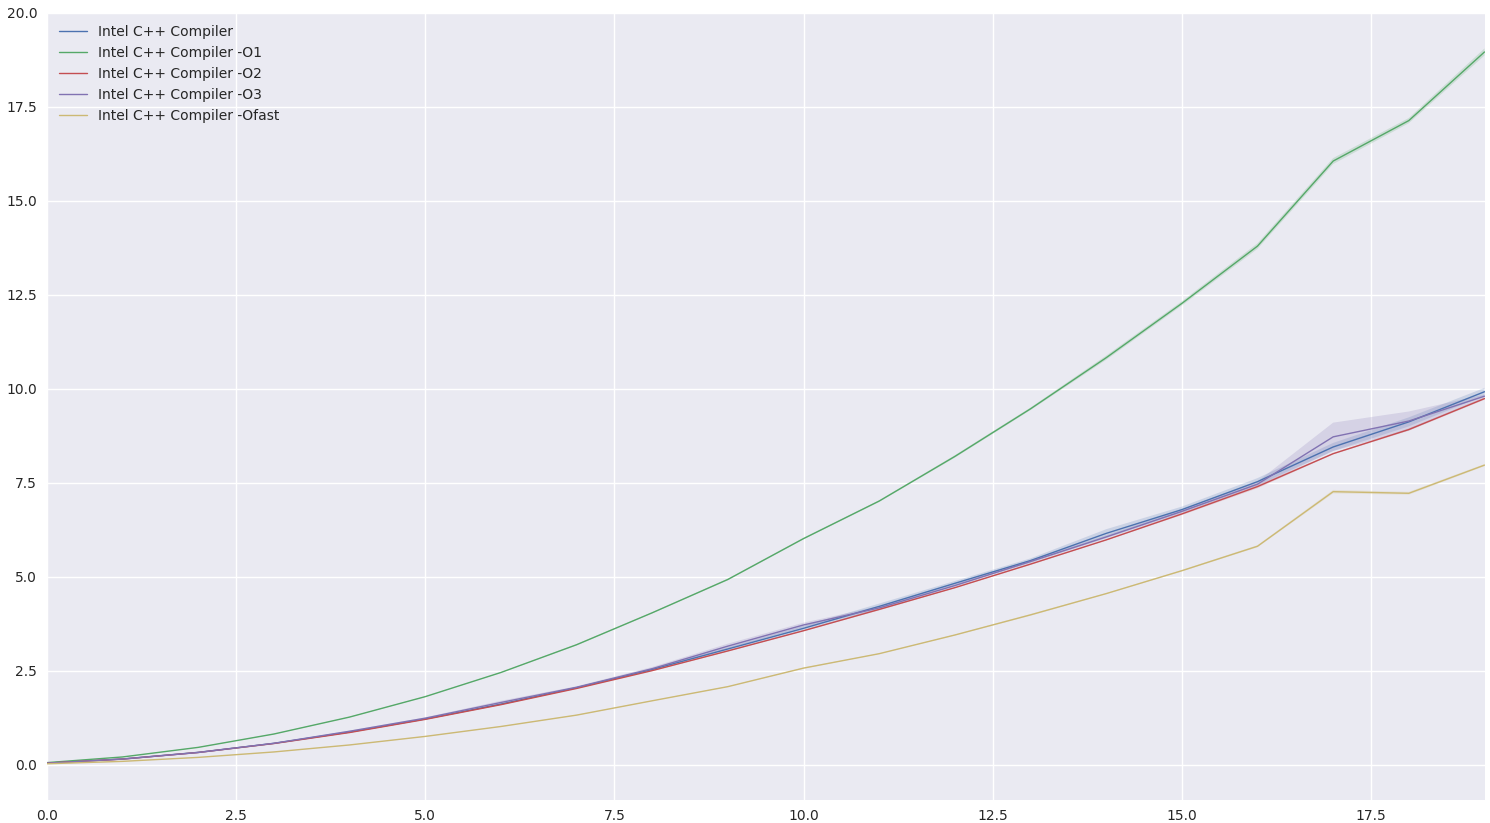
\includegraphics[width=\textwidth]{imagenes/plot_icc.png}
\end{figure}
~\\
~\\
Donde la versión mas optimizada de GCC daba un resultado para el tamaño de 20x20m, algo menor a 20s, el compilador ICC (Intel C++ compiler), muestra un tiempo de 10s, notablemente mas rápido que  GCC -Ofast, sin utilizar optimizaciónes. Esto se debe a que este compilador, como su nombre lo indica, fue diseñado para compilar para procesadores Intel, aprovechando las características específicas de los mismos. 
~\\
~\\
Se nota aquí otra diferencia, mientras que los flags llamados -Ox en GCC implementan siempre mejoras de velocidad de ejecución, el flag -O1, en ICC, busca mejorar el tamaño del ejecutable, dando así un tiempo de ejecución mayor que al no utilizar optimizaciónes. Notar que aún así, este es mas rapido que GCC -Ofast.
~\\
~\\
Finalmente, la mejor medida para ICC esta alrededor de los 8s.
~\\
~\\
\begin{figure}[H]
\caption{Tiempo(s) vs Tamaño(m) para Assembler(NASM)}
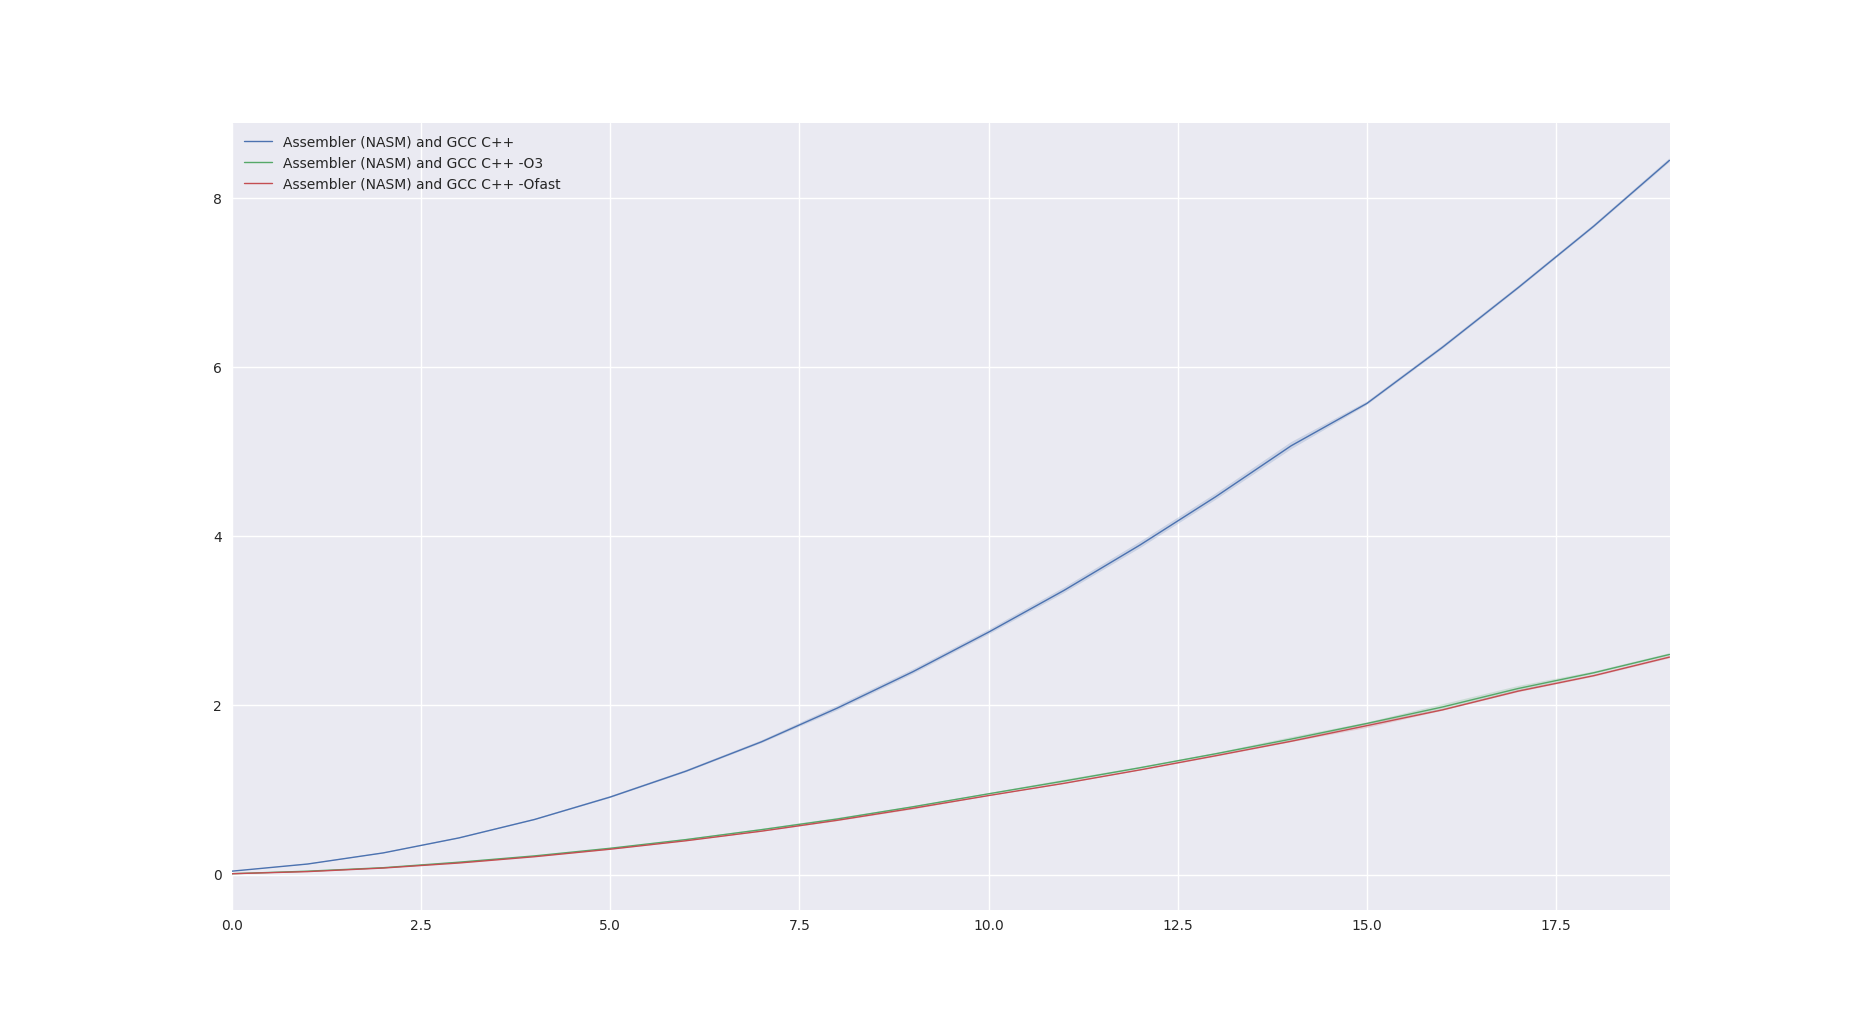
\includegraphics[width=\textwidth]{imagenes/plot_asm.png}
\end{figure}
~\\
~\\
De la misma forma en que GCC -Ofast tenia un rendimiento similar a ICC sin optimizaciónes, la versión producida en este trabajo, aprovechando la tecnología SIMD, tiene, sin optimizaciónes, un rendimiento similar a ICC -Ofast. Tambien muestra una mejora al utilizar flags, en particular llega a un tiempo de ejecusión poco mayor a 2s, al utilizar -O3 u -Ofast, optimizaciónes cuyas curvas son casi idénticas.
~\\
~\\
\begin{figure}[H]
\caption{Tiempo(s) vs Tamaño(m) para GCC + OpenMP}
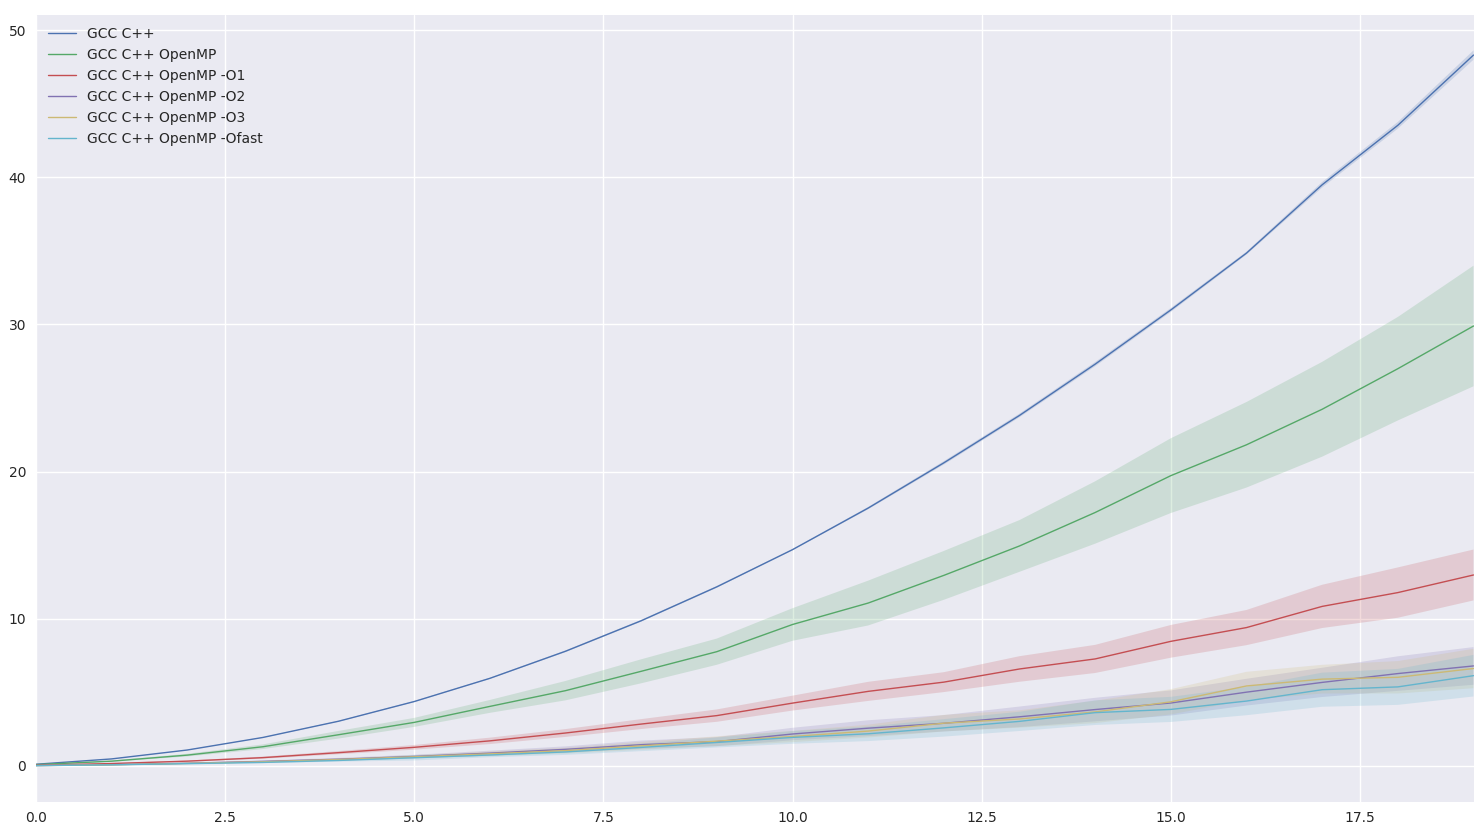
\includegraphics[width=\textwidth]{imagenes/plot_omp.png}
\end{figure}
Esta experimentación surje de una estrategia distinta, en lugar de intentar mejorar el rendimiento mediante la optimización de codigo por si sola, se intentara hacer lo mismo mediante la asignación de mayor cantidad de recursos computacionales. OpenMP es una tecnología que logra hacer esto de forma automatica. Se dispone, mediante OpenMP, de directivas que al aplicarla sobre un ciclo que depende de una variable, ejecuta distintas instancias del cuerpo del mismo en distintos núcleos del procesador, logrando paralelización a nivel CPU, reduciendo los tiempos de ejecición.
~\\
~\\
Dado que estamos agregando recursos computacionales, el uso de CPU aumenta, dejando pocos recursos para atender al resto de las tareas del sistema operativo. Se sospecha que este es el principal motivo, junto con la mayor catidad de cambios de contexto, para el aumento drastico de la varianza de las mediciónes respecto de los otros experimentos.
~\\
~\\
Notamos que aunque la asignación de mayor cantidad de recursos aumenta significativamente el rendimiento, este no supera a la versión SIMD. Hay una explicación razonable para este fenomeno, la maquina donde se realizó la experimentación, como se comentó anteriormente, utiliza un i7-920 2.67GHz. Este modelo de procesador dispone de 4 núcleos físicos, con lo cual OpenMP puede gracias a esto, dividir la tarea en 4 partes. La versión SIMD del programa, utiliza registros XMM, y valores flotantes de 32 bits de longitud, con lo cual logra, mediante vectorización, procesar 4 puntos de la malla al mismo tiempo. Siendo que ambas técnicas procesan un maximo teórico de 4 puntos de malla por cada ejecución del cuerpo del ciclo, y que SIMD no requiere comunicación entre distintos nucleos, este resulta en mejores prestaciónes.

\begin{figure}[H]
\caption{Tiempo(s) vs Tamaño(m) utilizando el flag -Ofast}
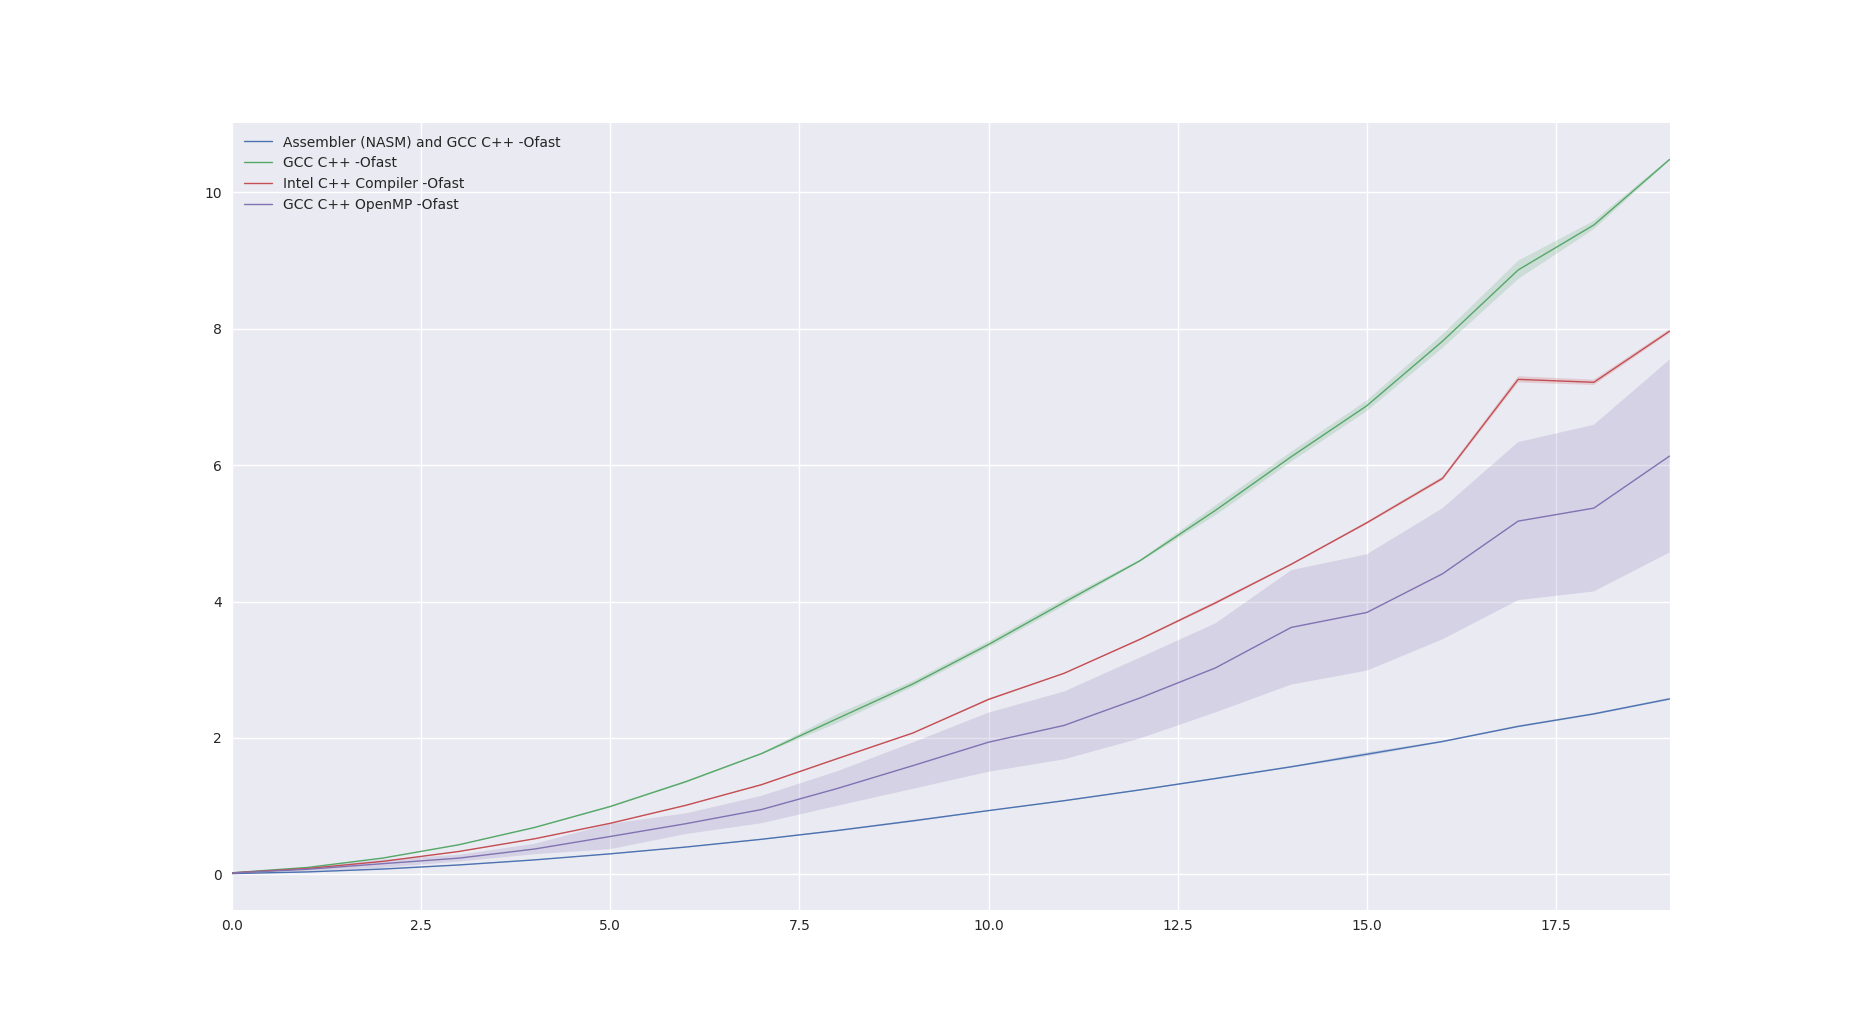
\includegraphics[width=\textwidth]{imagenes/plot_ofast.png}
\end{figure}

Por ultimo, y a modo ilustrativo, presentamos una gráfica de las optimizaciónes que dieron mejor resultado para cada técnica o compilador utilizado. En todos los casos el mejor rendimiento se obtuvo mediante la utilización del flag -Ofast. Queda claro mediante esta figura, que las mejores prestaciónes se dan al utilizar SIMD, seguido por OpenMP, ICC, y finalmente GCC. El patron queda claro, mientras mas recursos se utilizen, y mas especifico sea el codigo de acuerdo a la plataforma subyacente, mejor rendimiento se obtiene. 


\subsection{CPU vs. memoria}